%!TEX root =../../course-notes.tex
% ^ leave for LaTeXTools build functionality

\begin{readinessAssuranceOutcomes}
\item Determine if a system to a two-variable system of linear equations
      will have zero, one, or infinitely-many solutions by graphing.
\item Find the unique solution to a two-variable system of linear equations
      by back-substitution.
\end{readinessAssuranceOutcomes}

\begin{readinessAssuranceResources}
\item \url{https://www.khanacademy.org/math/cc-eighth-grade-math/cc-8th-systems-topic/cc-8th-systems-graphically/a/systems-of-equations-with-graphing}
\item \url{https://www.khanacademy.org/math/algebra/systems-of-linear-equations/solving-systems-of-equations-with-substitution/v/practice-using-substitution-for-systems}
\end{readinessAssuranceResources}




\begin{readinessAssuranceTest}

\item Which of these graphs represents the following system of linear equations?
      \begin{align*}
      x+2y   &=   4 \\
      2x-3y  &=  1
      \end{align*}

\begin{multicols}{4}
\begin{readinessAssuranceTestChoices}
\item
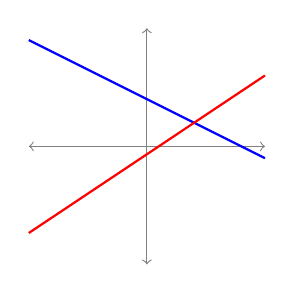
\begin{tikzpicture}[scale=0.3]
\draw[thin,gray,<->] (-5,0) -- (5,0);
\draw[thin,gray,<->] (0,-5) -- (0,5);
\draw[thick,blue] (-5,4.5) -- (5,-0.5);
\draw[thick,red] (-5,-3.67) -- (5,3);
\end{tikzpicture}
\item
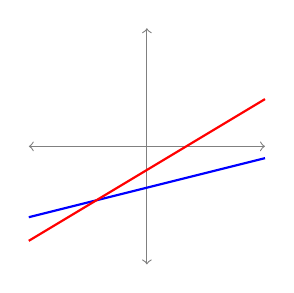
\begin{tikzpicture}[scale=0.3]
\draw[thin,gray,<->] (-5,0) -- (5,0);
\draw[thin,gray,<->] (0,-5) -- (0,5);
\draw[thick,blue] (-5,-3) -- (5,-0.5);
\draw[thick,red] (-5,-4) -- (5,2);
\end{tikzpicture}
\item
\begin{tikzpicture}[scale=0.3]
\draw[thin,gray,<->] (-5,0) -- (5,0);
\draw[thin,gray,<->] (0,-5) -- (0,5);
\draw[thick,purple] (-3,5) -- (5,-4);
\end{tikzpicture}
\item
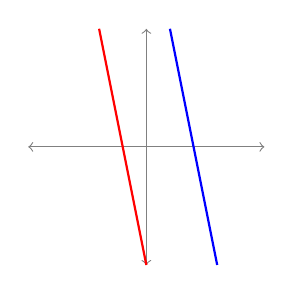
\begin{tikzpicture}[scale=0.3]
\draw[thin,gray,<->] (-5,0) -- (5,0);
\draw[thin,gray,<->] (0,-5) -- (0,5);
\draw[thick,blue] (3,-5) -- (1,5);
\draw[thick,red] (0,-5) -- (-2,5);
\end{tikzpicture}
\end{readinessAssuranceTestChoices}
\end{multicols}


\item How many solutions are there for the system of linear equations
      represented by the following graph?
    \begin{center}
      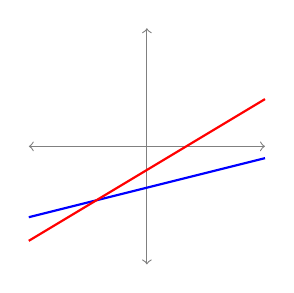
\begin{tikzpicture}[scale=0.3]
      \draw[thin,gray,<->] (-5,0) -- (5,0);
      \draw[thin,gray,<->] (0,-5) -- (0,5);
      \draw[thick,blue] (-5,-3) -- (5,-0.5);
      \draw[thick,red] (-5,-4) -- (5,2);
      \end{tikzpicture}
    \end{center}

\begin{multicols}{4}
\begin{readinessAssuranceTestChoices}
\item Zero
\item One
\item Two
\item Infinitely-many
\end{readinessAssuranceTestChoices}
\end{multicols}


\item How many solutions are there for the system of linear equations
      represented by the following graph? (This graph represents two completely
      overlapping lines.)
    \begin{center}
      \begin{tikzpicture}[scale=0.3]
      \draw[thin,gray,<->] (-5,0) -- (5,0);
      \draw[thin,gray,<->] (0,-5) -- (0,5);
      \draw[thick,purple] (-3,5) -- (5,-4);
      \end{tikzpicture}
    \end{center}

\begin{multicols}{4}
\begin{readinessAssuranceTestChoices}
\item Zero
\item One
\item Two
\item Infinitely-many
\end{readinessAssuranceTestChoices}
\end{multicols}


\item How many solutions are there for the system of linear equations
      represented by the following graph? (This graph represents two
      parallel lines.)
    \begin{center}
      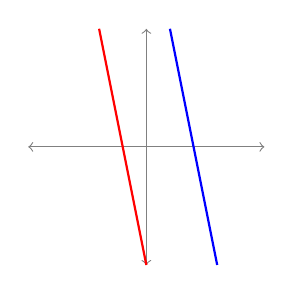
\begin{tikzpicture}[scale=0.3]
      \draw[thin,gray,<->] (-5,0) -- (5,0);
      \draw[thin,gray,<->] (0,-5) -- (0,5);
      \draw[thick,blue] (3,-5) -- (1,5);
      \draw[thick,red] (0,-5) -- (-2,5);
      \end{tikzpicture}
    \end{center}

\begin{multicols}{4}
\begin{readinessAssuranceTestChoices}
\item Zero
\item One
\item Two
\item Infinitely-many
\end{readinessAssuranceTestChoices}
\end{multicols}

\item Solve the following system of linear equations.
      \begin{align*}
      y   &=   2x+5 \\
      y  &=  -x+2
      \end{align*}

\begin{multicols}{4}
\begin{readinessAssuranceTestChoices}
\item \((x,y)=(-1,3)\)
\item \((x,y)=(4,-2)\)
\item There are no solutions.
\item There are infinitely-many solutions.
\end{readinessAssuranceTestChoices}
\end{multicols}

\item Solve the following system of linear equations.
      \begin{align*}
      x+2y   &=   4 \\
      2x-3y  &=  1
      \end{align*}

\begin{multicols}{4}
\begin{readinessAssuranceTestChoices}
\item \((x,y)=(-1,4)\)
\item \((x,y)=(2,1)\)
\item There are no solutions.
\item There are infinitely-many solutions.
\end{readinessAssuranceTestChoices}
\end{multicols}

\end{readinessAssuranceTest}
